%%
%% Copyright 2007-2020 Elsevier Ltd
%%
%% This file is part of the 'Elsarticle Bundle'.
%% ---------------------------------------------
%%
%% It may be distributed under the conditions of the LaTeX Project Public
%% License, either version 1.2 of this license or (at your option) any
%% later version.  The latest version of this license is in
%%    http://www.latex-project.org/lppl.txt
%% and version 1.2 or later is part of all distributions of LaTeX
%% version 1999/12/01 or later.
%%
%% The list of all files belonging to the 'Elsarticle Bundle' is
%% given in the file `manifest.txt'.
%%

%% Template article for Elsevier's document class `elsarticle'
%% with numbered style bibliographic references
%% SP 2008/03/01
%%
%%
%%
%% $Id: elsarticle-template-num.tex 190 2020-11-23 11:12:32Z rishi $
%%
%%
\documentclass[preprint,12pt]{elsarticle}

%% Use the option review to obtain double line spacing
%% \documentclass[authoryear,preprint,review,12pt]{elsarticle}

%% Use the options 1p,twocolumn; 3p; 3p,twocolumn; 5p; or 5p,twocolumn
%% for a journal layout:
%% \documentclass[final,1p,times]{elsarticle}
%% \documentclass[final,1p,times,twocolumn]{elsarticle}
%% \documentclass[final,3p,times]{elsarticle}
%% \documentclass[final,3p,times,twocolumn]{elsarticle}
%% \documentclass[final,5p,times]{elsarticle}
%% \documentclass[final,5p,times,twocolumn]{elsarticle}

%% For including figures, graphicx.sty has been loaded in
%% elsarticle.cls. If you prefer to use the old commands
%% please give \usepackage{epsfig}

%% The amssymb package provides various useful mathematical symbols
\usepackage{amssymb}
%% The amsthm package provides extended theorem environments
%% \usepackage{amsthm}
%% The amsmath package provides a handful of options for displaying equations.
\usepackage{amsmath}

%% The lineno packages adds line numbers. Start line numbering with
%% \begin{linenumbers}, end it with \end{linenumbers}. Or switch it on
%% for the whole article with \linenumbers.
\usepackage{lineno}

\journal{Physics Letters A}

\begin{document}

\begin{frontmatter}

%% Title, authors and addresses

%% use the tnoteref command within \title for footnotes;
%% use the tnotetext command for theassociated footnote;
%% use the fnref command within \author or \address for footnotes;
%% use the fntext command for theassociated footnote;
%% use the corref command within \author for corresponding author footnotes;
%% use the cortext command for theassociated footnote;
%% use the ead command for the email address,
%% and the form \ead[url] for the home page:
%% \title{Title\tnoteref{label1}}
%% \tnotetext[label1]{}
%% \author{Name\corref{cor1}\fnref{label2}}
%% \ead{email address}
%% \ead[url]{home page}
%% \fntext[label2]{}
%% \cortext[cor1]{}
%% \affiliation{organization={},
%%             addressline={},
%%             city={},
%%             postcode={},
%%             state={},
%%             country={}}
%% \fntext[label3]{}

\title{Multiple quantum NMR in solids as a method of a determination of Wigner--Yanase skew information}

%% use optional labels to link authors explicitly to addresses:
%% \author[label1,label2]{}
%% \affiliation[label1]{organization={},
%%             addressline={},
%%             city={},
%%             postcode={},
%%             state={},
%%             country={}}
%%
%% \affiliation[label2]{organization={},
%%             addressline={},
%%             city={},
%%             postcode={},
%%             state={},
%%             country={}}




\author[icp]{S.~I.~Doronin}
\author[icp]{E.~B.~Feldman}
\author[icp,msu]{I.~D.~Lazarev}
\address[icp]{Institute of Problems of Chemical Physics of Russian Academy of Sciences, \\ Chernogolovka, Moscow Region, Russia 142432}
\address[msu]{Faculty of Fundamental Physical-Chemical Engineering, Lomonosov Moscow State University, GSP-1, Moscow, Russia 119991}

\begin{abstract}
%% Text of abstract
A connection of the Wigner--Yanase skew information and multiple quantum (MQ) NMR coherences is considered at different temperatures and evolution times of nuclear spins with the dipole-dipole interactions in MQ NMR experiments in solids.
It is shown that the Wigner--Yanase skew information at temperature $T$ is equal to the doubled second moment of the MQ NMR spectra at the temperature twice large and any evolution times.
A comparison of the many--spin entanglement obtained with the Wigner--Yanase information and the Fisher information is conducted.
\end{abstract}

%%Graphical abstract
%\begin{graphicalabstract}
%\includegraphics{...}
%\end{graphicalabstract}

%%Research highlights
%\begin{highlights}
%\item Research highlight 1
%\item Research highlight 2
%\end{highlights}

\begin{keyword}
%% keywords here, in the form: keyword \sep keyword
multiple quantum (MQ) NMR \sep
%% PACS codes here, in the form: \PACS code \sep code
%\PACS 0000 \sep 1111
%%
%% MSC codes here, in the form: \MSC code \sep code
%% or \MSC[2008] code \sep code (2000 is the default)
%\MSC 0000 \sep 1111
\end{keyword}

\end{frontmatter}

\linenumbers

%% main text

\section{Introduction}
\label{sec:1}
The Wigner--Yanase skew information~\cite{1,2,3} together with the Fisher information~\cite{4,5} allow to develop the powerful methods for an investigation of entanglement, including the many--particle entanglement~\cite{6,7}.
Further investigations of the many--particle entanglement require a development of the corresponding experimental methods.
In particular, it was shown~\cite{6,8} that a low bound on the quantum Fisher information~\cite{4,5} coincides with the double second moment of the spectrum of multiple quantum (MQ) coherences.
As a result, the low bound on the quantum Fisher information can be found in MQ NMR experiments~\cite{9},
in cold--atom experiments, including Bose--Einstein condensates, ultracold atoms in cavities, and trapped ions~\cite{10,11,12,13,14}.
Using the properties of the quantum Fisher information one can obtain a number of entangled particles (spins) in the system under consideration~\cite{6} and even to find the dependence of a number of entangled spins on temperature~\cite{8}.


The Wigner--Yanase skew information~\cite{1,2,3} is also connected with the spectrum of MQ coherences.
In particular, we demonstrate in the present article that the Wigner--Yanase skew information in a spin system $(s = 1/2)$ with the dipole--dipole interactions (DDI) in MQ NMR experiment~\cite{9} at the system temperature $T$ equals to the double second moment of the MQ NMR spectrum obtained at temperature $2T$.
Using the properties of the Wigner--Yanase skew information one can investigate the many--spin entanglement on the basis of the MQ NMR spectroscopy~\cite{9}.


The main aim of the present article is a development of the method of extracting the Wigner--Yanase skew information from the MQ NMR spectra.
We also compare on the simple models~\cite{7,15} the many--spin entanglement obtained both with the Wigner--Yanase information and the Fisher information.


The article is organized as follows.
In Sec.~\ref{sec:2} the short introduction to the MQ NMR spectroscopy is given.
The connection of the Wigner--Yanase skew information with the second moment of the MQ NMR spectrum is obtained in Sec.~\ref{sec:3}.
A comparison of the many--spin entanglement obtained with Wigner--Yanase information and the Fisher information on the simple models~\cite{7,15} is conducted in Sec.~\ref{sec:4}.
We briefly discuss our results in the concluding Sec.~\ref{sec:5}.


\section{MQ NMR for solving problems of quantum informatics}
\label{sec:2}


\begin{figure}
	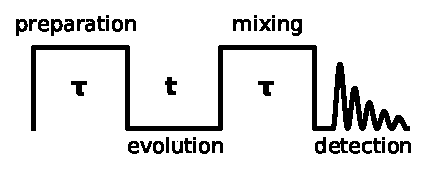
\includegraphics[width=0.95\linewidth]{mq-experiment}
	\caption{The basic scheme of the multiple quantum NMR experiment.}
	\label{fig:1}
\end{figure}

MQ NMR methods are widely used for solving problems of quantum informatics~\cite{16,17}. The MQ NMR experiment consists of four distinct periods of time Fig.~(\ref{fig:1}): preparation $(\tau)$, evolution $(t_1)$, mixing $(\tau)$, and detection $(t_2)$~\cite{9}.
MQ NMR coherences are created by a periodic multipulse sequence, consisting of
$\pm$-pulses, irradiating the system of the preparation period~\cite{9}.
If the inverse period of the multipulse sequence significantly exceeds the local dipolar field (in frequency units)~\cite{18}
MQ NMR dynamics can be described by the averaged nonsecular two--spin/two--quantum Hamiltonian~$H_{MQ}$
%
\begin{equation} \label{eq:1}
        H_{MQ} = H^{(+2)} + H^{(-2)} , \quad
        H^{(\pm 2)} = -\frac{1}{2} \sum_{j<k} D_{jk} I_{j} ^\pm I_k^\pm,
\end{equation}
%
where $D_{jk}$ is the coupling constant between spins $j$ and $k$, and $I_{j} ^+ I_k ^-$ are the raising and lowering operators of spin $j$.
On the mixing period the spin system is irradiated by the multiple sequence with $\pm y$--pulses.
As a result, the averaged nonsecular two-spin/two quantum Hamiltonian on the mixing period equals $(-H_{MQ})$~\cite{9}.


In order to investigate the MQ NMR dynamics of the system on the preparation period~\cite{9} one should find the density matrix $\rho(t)$ by solving the Liouville evolution equation~\cite{18}

\begin{equation}
    \label{eq:2}
        i\frac{d\rho(t)}{dt} = [H_{MQ}, \rho(t)]
\end{equation}
with the initial thermodynamic equilibrium density matrix
\begin{equation}
    \label{eq:3}
        \rho(0) = \rho_\mathrm{eq} = \frac{\exp(\frac{\hbar \omega_0}{kT}I_z)}{Z},
\end{equation}
where $Z=Tr \left\{exp\left(\frac{\hbar \omega_0}{kT}I_z\right) \right\}$ is the partition function, $\hbar$ and $k$ are the Pauli and Boltzmann constants, $\omega_0$ is the Larmor frequency, $T$ is the temperature, and $I_z$ is the operator of the projection of the total spin angular momentum on the $z$-axis, which is directed along the strong external magnetic field.


Following the preparation evolution and mixing periods of the MQ NMR experiments and taking into account the phase increment $\phi$ of the radio-frequency pulses~\cite{9}, the resulting signal $G(\tau,\phi)$ stored as population information is
%
\begin{equation} \label{eq:4}
	\begin{split}
		G(\tau,\phi)
		& = Tr \left\{
			e^{iH_{MQ}\tau} e^{i\phi I_z} e^{-iH_{MQ}\tau} \rho_\mathrm{eq}
			e^{iH_{MQ}\tau} e^{-i\phi I_z} e^{-iH_{MQ}\tau}\rho_\mathrm{eq}
		\right\}
		\\
		& = Tr \left\{
			e^{i\phi I_z} \rho_\mathrm{pre}(\tau,\beta)
      e^{-i\phi I_z}\rho_\mathrm{pre}(\tau,\beta)
		\right\},
	\end{split}
\end{equation}
%
where
%
\begin{equation} \label{eq:5}
	\rho_\mathrm{pre}(\tau,\beta) = e^{-iH_{MQ}\tau}\rho_\mathrm{eq}e^{iH_{MQ}\tau}
\end{equation}
%
is the density matrix at the end of the preparation period,
which can be defined from~Eqs.~(\ref{eq:2},\ref{eq:3}) and $\beta = \frac{\hbar \omega_0}{kT}$.


It is convenient to expand the density matrix $\rho_\mathrm{pre}(\tau)$ in series as~\cite{19}
\begin{equation}
    \label{eq:6}
        \rho_\mathrm{pre}(\tau,\beta) = \sum_n \rho_{\mathrm{pre},n}(\tau,\beta),
\end{equation}
where $\rho_\mathrm{pre}(\tau,\beta)$ is the contribution to the density matrix $\rho_\mathrm{pre}(\tau,\beta)$ from the MQ coherence of the n--th order.
Then the resulting signal $G(\tau,\phi)$ of the MQ NMR~\cite{9} can be rewritten as
\begin{equation} \label{eq:7}
    G(\tau, \phi) = \sum_n e^{in\phi}
        Tr\left\{\rho_{\mathrm{pre},n}(\tau,\beta)
        \rho_{\mathrm{pre},-n}(\tau,\beta) \right\},
\end{equation}
where we took into account that
\begin{equation}
    \label{eq:8}
        [I_z, \rho_{\mathrm{pre},n}] = n \rho_{\mathrm{pre},n}
\end{equation}
The normalized intensities of the MQ NMR coherences can be determined as follows
\begin{equation}
    \label{eq:9}
        J_n(\tau,\beta)= \frac{Tr\left\{\rho_{\mathrm{pre},n}(\tau,\beta)
            \rho_{\mathrm{pre},-n}(\tau,\beta)\right\}}
                {Tr(\rho^2_\mathrm{eq})}
\end{equation}
As was shown in~\cite{7},
\begin{equation}
    \label{eq:10}
        Tr(\rho_\mathrm{eq}^2) = \frac{2^N ch^N (\beta)}{Z^2}
\end{equation}
It was also shown that
\begin{equation}
    \label{eq:11}
        \sum_n J_n(\tau,\beta) = 1
\end{equation}
The second moment (dispersion) $M_2(\tau,\beta)$ of the distribution of the MQ NMR coherences $J_n (\tau,\beta)$ can be calculated from Eq.~(\ref{eq:7}) according to~\cite{20}
\begin{equation}
    \label{eq:12}
        M_2(\tau,\beta) = -\frac{1}{G_2(\tau,0)}
            \frac{d^2 G(t,\beta)}{dt^2}\bigg|
        _{t=0}
\end{equation}
Using Eqs.~(\ref{eq:7},\ref{eq:8},\ref{eq:12}) one can obtain
\begin{equation}
    \label{eq:13}
        M_2 (\tau,\beta) = \sum_n n^2 J_n(\tau,\beta)
\end{equation}
The low bound on the quantum Fisher information coincides with the double second moment of Eq.~(\ref{eq:13})~\cite{6,8}.
As a result, an analysis of the temperature dependence of the second moment $M_2(\tau,\beta)$ of the distribution of the intensities of the MQ NMR coherences allows us to obtain the number of entangled spins at different temperatures~\cite{7}.
In the following~Sec.~\ref{sec:3} we demonstrate that the Wigner--Yananse skew information is also connected with the second momentum $M_2(\tau,\beta)$
and can be useful for an investigation of the many-spin entanglement.

\section{The Wigner--Yanase skew information and MQ NMR}
\label{sec:3}
According definition~\cite{1,2} the Wigner--Yanase skew information
\begin{equation}
    \label{eq:14}
        I_{WY}(\rho(\tau,\beta),I_z) = -\frac{1}{2}
            Tr([\sqrt{\rho(\tau,\beta)},\sigma_z])^2 =
                -2Tr([\sqrt{\rho(\tau,\beta)},I_z])^2,
\end{equation}
where the Pauli operator $\sigma_z=2I_z$.
Introducing the evolution operator
\begin{equation}
    \label{eq:15}
        V(\tau) = e^{iH_{MQ}\tau}
\end{equation}
and using Eq.~(\ref{eq:3}) one can write the density matrix $\rho(\tau,\beta)$ as follows:
\begin{equation}
    \label{eq:16}
        \rho(\tau,\beta) = V^+(\tau) \frac{e^{\beta I_z}}{Z}V(\tau)
\end{equation}
Now we use te evident relationship:
\begin{equation}
    \label{eq:17}
        \sqrt{\rho(\tau,\beta)} =
            \sqrt{V^+(\tau)\frac{e^{\beta I_z}}{Z}V(\tau)} =
                V^+(\tau) \frac{e^{\frac{\beta}{2}}I_z}{\sqrt{Z}}V(\tau).
\end{equation}
It can be proved by simple calculation:
\begin{equation}
    \label{eq:18}
        \sqrt{\rho}\sqrt{\rho} =
            V^+(\tau)\frac{e^\frac{\beta}{2}I_z}{\sqrt{Z}}
                V(\tau)V^+(\tau)\frac{e^{\frac{\beta}{2}}I_z}{\sqrt{Z}}V(\tau) =
            V^+(\tau)\frac{e^\beta I_z}{Z}V(\tau) =
        \rho(\tau,\beta)
\end{equation}
%
Then we have
%
\begin{equation} \label{eq:19}
    \left[I_z,\sqrt{\rho(\tau,\beta)}\right]
    = \left[I_z, \sum_k \rho_k \left(\tau, \frac{\beta}{2}\right)\right]
    = \sum_k k\rho_k \left(\tau, \frac{\beta}{2}\right),
\end{equation}
%
and
%
\begin{equation} \label{eq:20}
	Tr\left[I_z,\sqrt{\rho(\tau,\beta)} \right]^2
	= Tr\left\{\sum_{k,k'}kk'
		\rho_k\left(\tau,\frac{\beta}{2}\right)
		\rho_k'\left(\tau,\frac{\beta}{2}\right)
	\right\}
	= \sum_k k^2 J_k\left(\tau,\frac{\beta}{2}\right).
\end{equation}
%
Finally, one can obtain that
%
\begin{equation} \label{eq:21}
    I_{WY}\left(\rho(\tau, \beta), I_z\right)
    = 2\sum_k k^2 J_k\left(\tau, \frac{\beta}{2}\right)
    = 2M_2\left(\tau, \frac{\beta}{2}\right)
\end{equation}
%
Thus, we obtain the important assertion.
If the spin system is investigated with MQ NMR at temperature $T\sim\beta^{-1}$ then the Wigner--Yanase skew information equals to the double second momentum of the distribution of the intensities of the MQ NMR coherences at temperature $2T \sim 2\beta^{-1}$ at any moment of the spin evolution.


The Wagner-Yanase skew information is connected with the second moment of the distribution of the MQ NMR coherences analogously to the Fisher information.
We compare these informations the following Section~\ref{sec:4}.


\section{A comparison of the many-spin entanglement obtained with the Wigner--Yanase information and the Fisher information}
\label{sec:4}

\begin{figure}
	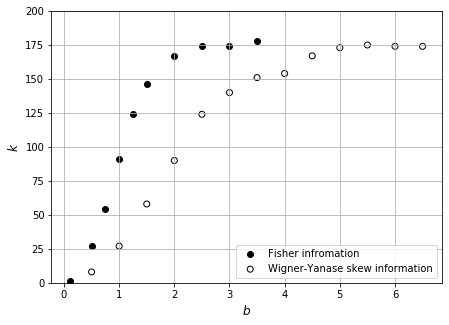
\includegraphics[width=0.95\linewidth]{entangled_spins_by_temp}
	\caption{
		The dependence of the number of the entangled spins on the inverse temperature $\beta = \frac{\pi \omega_0}{kT}$;
		black circles - the results are obtained with the Fisher information;
		open circles - the results are obtained with the Wigner--Yanase information.
	}
	\label{fig:2}
\end{figure}

The Wigner--Yanase skew information $I_{WY}(\rho(\tau,\beta),I_z)$ and the Fisher information $I_F(\rho(\tau,\beta),I_z)$ can be used for an investigation of the many-spin entanglement.
The informations are connected by the following restriction~\cite{3}
%
\begin{equation} \label{eq:22}
    I_{WY}\left(\rho(\tau,\beta), I_z\right)
    \leq I_F\left(\rho(\tau,\beta), I_z\right)
    \leq 2I_{WY}\left(\rho(\tau,\beta), I_z\right).
\end{equation}
%
For the comparison we used the model~\cite{21} of a nonspherical nanopore filled with a gas of spin-carrying atoms (for example, xenon) or molecules in a strong external magnetic field.
The restrictions (22) allow us to hope that the obtained results of the number of entangled spins are not strongly different.
This model allows to investigate the many-spin entanglement in the spin system consisting of hundreds of nuclear spins~\cite{7}.


We investigated the many-spin entanglement in the spin system, consisting of 201 spins, in a nanopore both with
the Wigner--Yanase information $I_{WY}\left(\rho(\tau, \beta), I_z\right)$
and the Fisher information $I_F\left(\rho(\tau,\beta),I_z\right)$.
In Fig.~(\ref{fig:2})the dependence of the number of entangled spins on the inverse temperature is presented.
Fig.~(\ref{fig:2}) demonstrates that the number of the entangled spins increases when the temperature decreases both for the Wigner--Yanase information and the Fisher information.


The analogous investigation was conducted on the model of the proton zigzag chain in a single crystal of hambergite~\cite{22}.
Here the close results on the many--spin entanglement were obtained for both used informations for the system consisting of $6\div 12$ spins.


\section{Conclusion}
\label{sec:5}

We studied the connection of the Wigner--Yanase skew information with the second moment of the distribution of the intensities of MQ coherences in the MQ NMR experiment.
It was shown that the Wigner--Yanase skew information at temperature $T \sim \beta^{-1}$ equals to the double second momentum of the MQ NMR spectrum at temperature $2T \sim 2\beta^{-1}$.
We compare also the results on the many--spin entanglement obtained with the Wigner--Yanase skew information and the Fisher information.


\section{Acknowledgement}
\label{sec:6}
We acknowledge funding from the Ministry of Science and Higher Education of the Russian Federation (Grant No.~075-15-2020-779).





%% The Appendices part is started with the command \appendix;
%% appendix sections are then done as normal sections
%\appendix
%\section{Sample Appendix Section}
%\label{sec:sample:appendix}
%Lorem ipsum dolor sit amet...

%% If you have bibdatabase file and want bibtex to generate the
%% bibitems, please use
%%
% \bibliographystyle{elsarticle-num}
% \bibliography{bibliography}

%% else use the following coding to input the bibitems directly in the
%% TeX file.

% \begin{thebibliography}{00}

% %% \bibitem{label}
% %% Text of bibliographic item

% \bibitem{}

% \end{thebibliography}

\begin{thebibliography}{20}
\bibitem{1} E.P.Wigner, M.M. Yanase, Proc.Nat.Acad.Sei. USA, 49, 910-918 (1963)
\bibitem{2} Z.Chen, Phys.Rev, A71, 052302 (2005)
\bibitem{3} S.Luo, Proc.Amer. Math.Soc.132, No.885-890 (2003)
\bibitem{4} G.Toth, I.Apellaniz, J. Phys. A47,424006 (2014)
\bibitem{5} L.Pezze, A.Smerzi, M.K. Oberthaler, R. Schmied, P.Treutlein, Rev.Mod.Phys. 90, 035005 (2018)
\bibitem{6} M.Gartner, P.Hauke, A.M.Rey, Phys.Rev.Lett. 120, 040402 (2018)
\bibitem{7} S.I.Doronin, E.B.Fel'dman, I.D.Lazarev, Phys. Rev. A100,022330 (2019)
\bibitem{8} D.Girolami, B.Yadin,Entropy 19,124 (2017)
\bibitem{9} J.Baum, M.Munowitz, A.N.Garroway, A.Pines,J.Chem.Phys. 83, 2015 (1985)
\bibitem{10} B. Swingle, G. Bentsen, M. Scheleier-Smith, P. Hayden, Phys. Rev. A94, 040302 (2010)
\bibitem{11} F.M. Cucchietti, J.Opt.Soc. Am. B27, A30 (2010)
\bibitem{12} I.D. Leroux, M.H. Schleirer-Smith, V.Vuletii, Phys.Rev.Lett. 104,
	073602 (2010)

\bibitem{13} T.Macri, A. Smerzi, L.Pezze, Phys.Rev F94, 010102 (2016)
\bibitem{14} M.Gartner, J.G.Bohnet, A.Safavi-Naini, M.L. Wall, J.J. Bollinger, A.M.Rey, Nat.Phys. 13,781 (2017)
\bibitem{15} G.A.Bochkin, S.G.Vesil'ev, S.I. Doronin, E.I.Kuznetsova,I.D.Lazarev,E.B.Fel'dman, Appl.Magn.Reson. 51,667-678 (2020)
\bibitem{16} E.B.Fel'dman, A.N. Pykov, A.I.Zenchuk, Philos. Trans. R. Soc. London A370, 4690 (2012)
\bibitem{17} G.B.Furman, V.M.Meerovich, V.L.Sokoovsky, Phys. Rev. A.78 042301 (2008)
\bibitem{18} M.Goldman. Spin temperature and nuclear magnetic resonance in solids, Oxford,UK, Clarendon Press. 1970.
\bibitem{19} E.B.Fel'dman, S.Lacelle,Chem.Phys.Lett. 253, 27 (1996)
\bibitem{20} A.Abragam, The Princioles of Nuclear Magnetism, Clarendon. Oxford. 1961
\bibitem{21} J. Baugh, A. Kleinhammes, D. Han, Q. Wang, Y.Wn, Science 294, 1505 (2001)
\bibitem{22} G.A. Bochkin, E.B. Fel'dman, E.B. Kuznetsova, I.D. Lasarev, S.G. Vasil'ev, V.I.Volkov, J. Magn.Reson. 319, 106816 (2020)
\end{thebibliography}

\end{document}
\endinput
